\tikzstyle{obj1}=[black, line width = 0.7pt, line join=round, line cap=round]
\tikzstyle{obj2}=[BrickRed, line width = 0.7pt, line join=round, line cap=round]
\tikzstyle{obj3}=[BlueViolet!80, line width = .7pt, line join=round, line cap=round]
\tikzset{wiggly/.style={decorate, decoration={snake, segment length=4.1pt, amplitude=1.pt}}}

\newcommand{\middleCoo}[3]{
    \path (#1) --coordinate[pos=0.5](#3) (#2);
}

\tikzset{->-/.style={decoration={
        markings,
        mark=at position #1 with {\arrow{Triangle[width=3pt, length=3pt]}}},postaction={decorate}}}

\tikzset{-<-/.style={decoration={
        markings,
        mark=at position #1 with {\arrowreversed{Triangle[width=3pt, length=3pt]}}}}}

\tikzset{mpoint/.style={ transform shape, sloped, 
minimum width=20pt, minimum height=3pt, inner sep=0pt, ultra thin, font=\tiny}}

\tikzset{
    clip even odd rule/.code={\pgfseteorule},
    invclip/.style={clip,insert path=[clip even odd rule]{
    [reset cm](-\maxdimen,-\maxdimen)rectangle(\maxdimen,\maxdimen)
}}}

\newcommand{\trianglePts}[4]{
    \def\shr{#4};
    \middleCoo{#1}{#2}{#1#2};
    \middleCoo{#2}{#3}{#2#3};
    \middleCoo{#1}{#3}{#1#3};
    \coordinate (#1#1#2) at ($(#1)!\shr!(#1#2)$);
    \coordinate (#1#2#2) at ($(#2)!\shr!(#1#2)$);
    \coordinate (#2#2#3) at ($(#2)!\shr!(#2#3)$);
    \coordinate (#2#3#3) at ($(#3)!\shr!(#2#3)$);
    \coordinate (#1#1#3) at ($(#1)!\shr!(#1#3)$);
    \coordinate (#1#3#3) at ($(#3)!\shr!(#1#3)$);
    \path[name path=P#1] (#1) -- (#2#3);
    \path[name path=P#2] (#2) -- (#1#3);
    \path[name path=P#3] (#3) -- (#1#2);
    \path[name intersections={of=P#1 and P#2,by={#1#2#3}}];
    \coordinate (#1#1#2#3) at ($(#1)!\shr!(#1#2#3)$);
    \coordinate (#2#1#2#3) at ($(#2)!\shr!(#1#2#3)$);
    \coordinate (#3#1#2#3) at ($(#3)!\shr!(#1#2#3)$);
}

\newcommand\clipIntersection[1]{
    (#1.north west) -- (#1.north east) -- (#1.south east) -- (#1.south west) -- (#1.north west)
}

\newcommand\clipAroundTwoNodes[3]{
    \begin{pgfscope}
        \begin{scope}[overlay]
            \path[invclip] \clipIntersection{#1} \clipIntersection{#2};#3
        \end{scope}
    \end{pgfscope}
}

\newcommand\clipAroundFourNodes[5]{
    \begin{pgfscope}
        \begin{scope}[overlay]
            \path[invclip] \clipIntersection{#1} \clipIntersection{#2} \clipIntersection{#3} \clipIntersection{#4};#5
        \end{scope}
    \end{pgfscope}
}

\newcommand\FerroFade[1]{%
\begin{tikzpicture}[
	baseline={(current bounding box.center)}
	]
	
	\def\l{.6}
	\def\v{#1}
	\def\tc{6}     % Tc lies between magnet \tc-1 and magnet \tc
	\def\R{.36}    % outer radius of the horseshoe
	\def\r{.12}    % inner radius of the horseshoe
	\def\h{.55}    % length of the legs
	\def\t{.18}    % length of the white pole tips
	
	% Outline of a chubby horseshoe magnet, opening downwards, with rounded feet
	\def\horseshoe{[rounded corners={.07*\l*1cm}] ({-\R*\l},{-\h*\l}) -- ({-\R*\l},0) arc[start angle=180, end angle=0, radius={\R*\l}]
		-- ({\R*\l},{-\h*\l}) -- ({\r*\l},{-\h*\l}) -- ({\r*\l},0) arc[start angle=0, end angle=180, radius={\r*\l}]
		-- ({-\r*\l},{-\h*\l}) -- cycle}
	
	% Horseshoe magnets fading out in equal steps up to Tc, grey above Tc
	\foreach \k in {0,...,9} {
		\pgfmathsetmacro\m{max(1-\k/\tc,0)}
		\begin{scope}[shift={({(\k+.5)*\l},{1.2*\l})}]
			\begin{scope}
				\clip \horseshoe;
				\fill[gray!30] ({-\R*\l},{-\h*\l}) rectangle ({\R*\l},{\R*\l});
				\fill[red, fill opacity=\m] ({-\R*\l},{-\h*\l}) rectangle (0,{\R*\l});
				\fill[UGentBlue, fill opacity=\m] (0,{-\h*\l}) rectangle ({\R*\l},{\R*\l});
				\fill[white] ({-\R*\l},{-\h*\l}) rectangle ({\R*\l},{(\t-\h)*\l});
			\end{scope}
			\draw[obj1] \horseshoe;
			\draw[obj1] ({-\R*\l},{(\t-\h)*\l}) -- ({-\r*\l},{(\t-\h)*\l});
			\draw[obj1] ({\r*\l},{(\t-\h)*\l}) -- ({\R*\l},{(\t-\h)*\l});
			% little shine on the arch
			\draw[white, line width=1pt, line cap=round] (145:{.24*\l}) arc[start angle=145, end angle=110, radius={.24*\l}];
		\end{scope}
	}
	
	% Temperature axis
	\draw[obj1, -{Latex}] (0,0) -- ({10.5*\l},0) node[right] {$T$};
	\draw[obj1] ({\tc*\l},{-.15*\l}) -- ({\tc*\l},{.15*\l}) node[below=4pt] {$T_c$};
	
	% Both phases are stable
	\ifnum\v>0
		\node[below=4pt] at ({\tc/2*\l},{.15*\l}) {stable};
		\node[below=4pt] at ({(\tc+10)/2*\l},{.15*\l}) {stable};
	\fi
	
\end{tikzpicture}}

\newcommand{\magnet}[3]{\tikz[baseline=-0.55ex]{%
  \def\s{0.45em}
  \path (-0.65*\s,0) (0.65*\s,0);
  \begin{scope}[rotate=#1-90]
    \fill[#2] (-0.45*\s,0) -- (0,\s)  -- (0.45*\s,0) -- cycle;
    \fill[#3] (-0.45*\s,0) -- (0,-\s) -- (0.45*\s,0) -- cycle;
    \draw[obj1, line join=round] (0,\s) -- (0.45*\s,0) -- (0,-\s) -- (-0.45*\s,0) -- cycle;
  \end{scope}}}
\newcommand{\spinup}{\magnet{90}{red}{UGentBlue}}
\newcommand{\spindown}{\magnet{-90}{red}{UGentBlue}}
\newcommand{\spinleft}{\magnet{0}{red}{UGentBlue}}
\newcommand{\spinright}{\magnet{180}{red}{UGentBlue}}
\newcommand{\spinsuper}{\magnet{90}{red!50!UGentBlue}{purple}}

\newcommand{\DiamondUnitCell}{
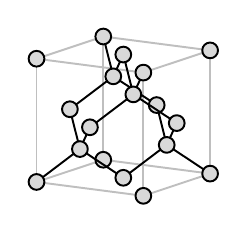
\begin{tikzpicture}[
	baseline={(current bounding box.center)}
	]
	
	\def\l{.4}
	\def\r{.25} % radius of the atoms
	\def\a{32}   % azimuth
	\def\e{12}   % elevation
	
	% Conventional cubic cell of side 4. Atoms and bonds are listed from back to front
	% for this view; after a large change of \a or \e the order has to be redone.
	\begin{scope}[
		x={({cos(\a)*\l*1cm},{-sin(\a)*sin(\e)*\l*1cm})},
		y={({sin(\a)*\l*1cm},{cos(\a)*sin(\e)*\l*1cm})},
		z={(0,{cos(\e)*\l*1cm})},
		atom/.style={obj1, fill=gray!30},
		bond/.style={obj1, shorten <={\r*\l*1cm}, shorten >={\r*\l*1cm}}
		]
		
		% Edges of the cube
		\foreach \p/\q in {{0,0,0}/{0,0,4}, {0,0,0}/{0,4,0}, {0,0,0}/{4,0,0}, {0,0,4}/{0,4,4}, {0,0,4}/{4,0,4}, {0,4,0}/{0,4,4}, {0,4,0}/{4,4,0}, {0,4,4}/{4,4,4}, {4,0,0}/{4,0,4}, {4,0,0}/{4,4,0}, {4,0,4}/{4,4,4}, {4,4,0}/{4,4,4}} {
			\draw[obj1, gray!50] (\p) -- (\q);
		}
		
		\filldraw[atom] (0,4,0) circle ({\r*\l*1cm});
		\filldraw[atom] (0,4,4) circle ({\r*\l*1cm});
		\draw[bond] (1,3,3) -- (0,4,4);
		\filldraw[atom] (2,4,2) circle ({\r*\l*1cm});
		\draw[bond] (1,3,3) -- (2,4,2);
		\filldraw[atom] (1,3,3) circle ({\r*\l*1cm});
		\draw[bond] (3,3,1) -- (2,4,2);
		\draw[bond] (1,3,3) -- (0,2,2);
		\filldraw[atom] (4,4,0) circle ({\r*\l*1cm});
		\filldraw[atom] (0,2,2) circle ({\r*\l*1cm});
		\draw[bond] (3,3,1) -- (4,4,0);
		\filldraw[atom] (3,3,1) circle ({\r*\l*1cm});
		\draw[bond] (3,3,1) -- (2,2,0);
		\draw[bond] (1,1,1) -- (0,2,2);
		\filldraw[atom] (2,2,0) circle ({\r*\l*1cm});
		\draw[bond] (1,3,3) -- (2,2,4);
		\filldraw[atom] (4,4,4) circle ({\r*\l*1cm});
		\draw[bond] (1,1,1) -- (2,2,0);
		\filldraw[atom] (1,1,1) circle ({\r*\l*1cm});
		\draw[bond] (1,1,1) -- (0,0,0);
		\filldraw[atom] (0,0,0) circle ({\r*\l*1cm});
		\draw[bond] (3,3,1) -- (4,2,2);
		\filldraw[atom] (2,2,4) circle ({\r*\l*1cm});
		\draw[bond] (1,1,1) -- (2,0,2);
		\draw[bond] (3,1,3) -- (2,2,4);
		\filldraw[atom] (4,2,2) circle ({\r*\l*1cm});
		\filldraw[atom] (0,0,4) circle ({\r*\l*1cm});
		\draw[bond] (3,1,3) -- (4,2,2);
		\filldraw[atom] (3,1,3) circle ({\r*\l*1cm});
		\draw[bond] (3,1,3) -- (2,0,2);
		\filldraw[atom] (2,0,2) circle ({\r*\l*1cm});
		\filldraw[atom] (4,0,0) circle ({\r*\l*1cm});
		\draw[bond] (3,1,3) -- (4,0,4);
		\filldraw[atom] (4,0,4) circle ({\r*\l*1cm});
		
	\end{scope}
	
\end{tikzpicture}
}

\newcommand{\CalciteUnitCell}{
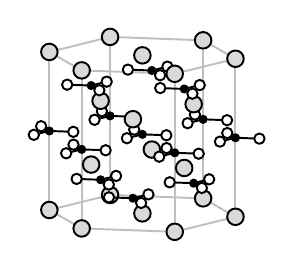
\begin{tikzpicture}[
	baseline={(current bounding box.center)}
	]
	
	\def\l{.3}
	\def\rca{.35}  % radius of Ca
	\def\rc{.15}   % radius of C
	\def\ro{.22}   % radius of O
	\def\a{10}     % azimuth
	\def\e{12}     % elevation
	
	% Calcite (R-3c) in a hexagonal prism of three hexagonal cells, lower half (0 <= z <= c/2), c-axis vertical.
	% a = 4.99, c = 17.06 Angstrom, drawn with 4 units per a.
	% Ca (grey), C (black) and O (white); every CO3 group is a flat triangle perpendicular to c.
	% Atoms and bonds are listed from back to front for this view.
	\begin{scope}[
		x={({cos(\a)*\l*1cm},{-sin(\a)*sin(\e)*\l*1cm})},
		y={({sin(\a)*\l*1cm},{cos(\a)*sin(\e)*\l*1cm})},
		z={(0,{cos(\e)*\l*1cm})},
		ca/.style={obj1, fill=gray!30},
		carbon/.style={obj1, fill=black},
		oxygen/.style={obj1, fill=white},
		bond/.style={obj1, shorten <={\rc*\l*1cm}, shorten >={\ro*\l*1cm}}
		]
		
		% Edges of the cell
		\foreach \p/\q in {{4.00,0.00,0.00}/{2.00,3.46,0.00}, {4.00,0.00,6.84}/{2.00,3.46,6.84}, {4.00,0.00,0.00}/{4.00,0.00,6.84}, {2.00,3.46,0.00}/{-2.00,3.46,0.00}, {2.00,3.46,6.84}/{-2.00,3.46,6.84}, {2.00,3.46,0.00}/{2.00,3.46,6.84}, {-2.00,3.46,0.00}/{-4.00,0.00,0.00}, {-2.00,3.46,6.84}/{-4.00,0.00,6.84}, {-2.00,3.46,0.00}/{-2.00,3.46,6.84}, {-4.00,0.00,0.00}/{-2.00,-3.46,0.00}, {-4.00,0.00,6.84}/{-2.00,-3.46,6.84}, {-4.00,0.00,0.00}/{-4.00,0.00,6.84}, {-2.00,-3.46,0.00}/{2.00,-3.46,0.00}, {-2.00,-3.46,6.84}/{2.00,-3.46,6.84}, {-2.00,-3.46,0.00}/{-2.00,-3.46,6.84}, {2.00,-3.46,0.00}/{4.00,0.00,0.00}, {2.00,-3.46,6.84}/{4.00,0.00,6.84}, {2.00,-3.46,0.00}/{2.00,-3.46,6.84}} {
			\draw[obj1, gray!50] (\p) -- (\q);
		}
		
		\filldraw[oxygen] (-2.51,4.35,3.42) circle ({\ro*\l*1cm});
		\filldraw[ca] (-2.00,3.46,0.00) circle ({\rca*\l*1cm});
		\draw[bond] (-2.00,3.46,3.42) -- (-2.51,4.35,3.42);
		\filldraw[oxygen] (1.49,4.35,3.42) circle ({\ro*\l*1cm});
		\filldraw[ca] (2.00,3.46,0.00) circle ({\rca*\l*1cm});
		\filldraw[carbon] (-2.00,3.46,3.42) circle ({\rc*\l*1cm});
		\draw[bond] (-2.00,3.46,3.42) -- (-0.97,3.46,3.42);
		\filldraw[oxygen] (-0.97,3.46,3.42) circle ({\ro*\l*1cm});
		\draw[bond] (2.00,3.46,3.42) -- (1.49,4.35,3.42);
		\draw[bond] (-2.00,3.46,3.42) -- (-2.51,2.57,3.42);
		\filldraw[carbon] (2.00,3.46,3.42) circle ({\rc*\l*1cm});
		\filldraw[ca] (-2.00,3.46,6.84) circle ({\rca*\l*1cm});
		\draw[bond] (2.00,3.46,3.42) -- (3.03,3.46,3.42);
		\filldraw[oxygen] (-2.51,2.57,3.42) circle ({\ro*\l*1cm});
		\filldraw[oxygen] (3.03,3.46,3.42) circle ({\ro*\l*1cm});
		\filldraw[oxygen] (-1.49,2.04,1.14) circle ({\ro*\l*1cm});
		\draw[bond] (2.00,3.46,3.42) -- (1.49,2.57,3.42);
		\filldraw[oxygen] (0.51,3.20,5.70) circle ({\ro*\l*1cm});
		\filldraw[ca] (0.00,2.31,2.28) circle ({\rca*\l*1cm});
		\draw[bond] (-2.00,1.15,1.14) -- (-1.49,2.04,1.14);
		\filldraw[ca] (2.00,3.46,6.84) circle ({\rca*\l*1cm});
		\filldraw[oxygen] (1.49,2.57,3.42) circle ({\ro*\l*1cm});
		\draw[bond] (0.00,2.31,5.70) -- (0.51,3.20,5.70);
		\filldraw[oxygen] (-3.03,1.15,1.14) circle ({\ro*\l*1cm});
		\filldraw[oxygen] (2.51,2.04,1.14) circle ({\ro*\l*1cm});
		\draw[bond] (-2.00,1.15,1.14) -- (-3.03,1.15,1.14);
		\filldraw[carbon] (-2.00,1.15,1.14) circle ({\rc*\l*1cm});
		\filldraw[oxygen] (-1.03,2.31,5.70) circle ({\ro*\l*1cm});
		\draw[bond] (0.00,2.31,5.70) -- (-1.03,2.31,5.70);
		\filldraw[carbon] (0.00,2.31,5.70) circle ({\rc*\l*1cm});
		\draw[bond] (2.00,1.15,1.14) -- (2.51,2.04,1.14);
		\filldraw[oxygen] (-4.51,0.89,3.42) circle ({\ro*\l*1cm});
		\draw[bond] (-2.00,1.15,1.14) -- (-1.49,0.26,1.14);
		\filldraw[oxygen] (0.97,1.15,1.14) circle ({\ro*\l*1cm});
		\filldraw[ca] (-4.00,0.00,0.00) circle ({\rca*\l*1cm});
		\draw[bond] (2.00,1.15,1.14) -- (0.97,1.15,1.14);
		\draw[bond] (0.00,2.31,5.70) -- (0.51,1.42,5.70);
		\filldraw[carbon] (2.00,1.15,1.14) circle ({\rc*\l*1cm});
		\filldraw[ca] (-2.00,1.15,4.56) circle ({\rca*\l*1cm});
		\draw[bond] (-4.00,0.00,3.42) -- (-4.51,0.89,3.42);
		\filldraw[oxygen] (-1.49,0.26,1.14) circle ({\ro*\l*1cm});
		\filldraw[oxygen] (-0.51,0.89,3.42) circle ({\ro*\l*1cm});
		\filldraw[oxygen] (0.51,1.42,5.70) circle ({\ro*\l*1cm});
		\draw[bond] (2.00,1.15,1.14) -- (2.51,0.26,1.14);
		\filldraw[ca] (0.00,0.00,0.00) circle ({\rca*\l*1cm});
		\filldraw[carbon] (-4.00,0.00,3.42) circle ({\rc*\l*1cm});
		\draw[bond] (-4.00,0.00,3.42) -- (-2.97,0.00,3.42);
		\filldraw[ca] (2.00,1.15,4.56) circle ({\rca*\l*1cm});
		\filldraw[oxygen] (-2.97,0.00,3.42) circle ({\ro*\l*1cm});
		\draw[bond] (0.00,0.00,3.42) -- (-0.51,0.89,3.42);
		\filldraw[oxygen] (2.51,0.26,1.14) circle ({\ro*\l*1cm});
		\draw[bond] (-4.00,0.00,3.42) -- (-4.51,-0.89,3.42);
		\filldraw[oxygen] (3.49,0.89,3.42) circle ({\ro*\l*1cm});
		\filldraw[ca] (4.00,0.00,0.00) circle ({\rca*\l*1cm});
		\filldraw[carbon] (0.00,0.00,3.42) circle ({\rc*\l*1cm});
		\filldraw[ca] (-4.00,0.00,6.84) circle ({\rca*\l*1cm});
		\draw[bond] (0.00,0.00,3.42) -- (1.03,0.00,3.42);
		\filldraw[oxygen] (-4.51,-0.89,3.42) circle ({\ro*\l*1cm});
		\filldraw[oxygen] (1.03,0.00,3.42) circle ({\ro*\l*1cm});
		\draw[bond] (4.00,0.00,3.42) -- (3.49,0.89,3.42);
		\draw[bond] (0.00,0.00,3.42) -- (-0.51,-0.89,3.42);
		\filldraw[oxygen] (-1.49,-0.26,5.70) circle ({\ro*\l*1cm});
		\filldraw[ca] (-2.00,-1.15,2.28) circle ({\rca*\l*1cm});
		\filldraw[carbon] (4.00,0.00,3.42) circle ({\rc*\l*1cm});
		\filldraw[ca] (0.00,0.00,6.84) circle ({\rca*\l*1cm});
		\draw[bond] (4.00,0.00,3.42) -- (5.03,0.00,3.42);
		\filldraw[oxygen] (-0.51,-0.89,3.42) circle ({\ro*\l*1cm});
		\filldraw[oxygen] (5.03,0.00,3.42) circle ({\ro*\l*1cm});
		\draw[bond] (-2.00,-1.15,5.70) -- (-1.49,-0.26,5.70);
		\filldraw[oxygen] (0.51,-1.42,1.14) circle ({\ro*\l*1cm});
		\draw[bond] (4.00,0.00,3.42) -- (3.49,-0.89,3.42);
		\filldraw[oxygen] (-3.03,-1.15,5.70) circle ({\ro*\l*1cm});
		\filldraw[oxygen] (2.51,-0.26,5.70) circle ({\ro*\l*1cm});
		\draw[bond] (-2.00,-1.15,5.70) -- (-3.03,-1.15,5.70);
		\filldraw[ca] (2.00,-1.15,2.28) circle ({\rca*\l*1cm});
		\filldraw[carbon] (-2.00,-1.15,5.70) circle ({\rc*\l*1cm});
		\draw[bond] (0.00,-2.31,1.14) -- (0.51,-1.42,1.14);
		\filldraw[ca] (4.00,0.00,6.84) circle ({\rca*\l*1cm});
		\filldraw[oxygen] (3.49,-0.89,3.42) circle ({\ro*\l*1cm});
		\draw[bond] (2.00,-1.15,5.70) -- (2.51,-0.26,5.70);
		\filldraw[oxygen] (-1.03,-2.31,1.14) circle ({\ro*\l*1cm});
		\draw[bond] (0.00,-2.31,1.14) -- (-1.03,-2.31,1.14);
		\draw[bond] (-2.00,-1.15,5.70) -- (-1.49,-2.04,5.70);
		\filldraw[carbon] (0.00,-2.31,1.14) circle ({\rc*\l*1cm});
		\filldraw[oxygen] (0.97,-1.15,5.70) circle ({\ro*\l*1cm});
		\draw[bond] (2.00,-1.15,5.70) -- (0.97,-1.15,5.70);
		\filldraw[carbon] (2.00,-1.15,5.70) circle ({\rc*\l*1cm});
		\filldraw[oxygen] (-2.51,-2.57,3.42) circle ({\ro*\l*1cm});
		\filldraw[oxygen] (-1.49,-2.04,5.70) circle ({\ro*\l*1cm});
		\draw[bond] (0.00,-2.31,1.14) -- (0.51,-3.20,1.14);
		\filldraw[ca] (-2.00,-3.46,0.00) circle ({\rca*\l*1cm});
		\draw[bond] (2.00,-1.15,5.70) -- (2.51,-2.04,5.70);
		\filldraw[ca] (0.00,-2.31,4.56) circle ({\rca*\l*1cm});
		\draw[bond] (-2.00,-3.46,3.42) -- (-2.51,-2.57,3.42);
		\filldraw[oxygen] (0.51,-3.20,1.14) circle ({\ro*\l*1cm});
		\filldraw[oxygen] (1.49,-2.57,3.42) circle ({\ro*\l*1cm});
		\filldraw[oxygen] (2.51,-2.04,5.70) circle ({\ro*\l*1cm});
		\filldraw[ca] (2.00,-3.46,0.00) circle ({\rca*\l*1cm});
		\filldraw[carbon] (-2.00,-3.46,3.42) circle ({\rc*\l*1cm});
		\draw[bond] (-2.00,-3.46,3.42) -- (-0.97,-3.46,3.42);
		\filldraw[oxygen] (-0.97,-3.46,3.42) circle ({\ro*\l*1cm});
		\draw[bond] (2.00,-3.46,3.42) -- (1.49,-2.57,3.42);
		\draw[bond] (-2.00,-3.46,3.42) -- (-2.51,-4.35,3.42);
		\filldraw[carbon] (2.00,-3.46,3.42) circle ({\rc*\l*1cm});
		\filldraw[ca] (-2.00,-3.46,6.84) circle ({\rca*\l*1cm});
		\draw[bond] (2.00,-3.46,3.42) -- (3.03,-3.46,3.42);
		\filldraw[oxygen] (-2.51,-4.35,3.42) circle ({\ro*\l*1cm});
		\filldraw[oxygen] (3.03,-3.46,3.42) circle ({\ro*\l*1cm});
		\draw[bond] (2.00,-3.46,3.42) -- (1.49,-4.35,3.42);
		\filldraw[ca] (2.00,-3.46,6.84) circle ({\rca*\l*1cm});
		\filldraw[oxygen] (1.49,-4.35,3.42) circle ({\ro*\l*1cm});
		
	\end{scope}
	
\end{tikzpicture}
}

\newcommand\sterngerlach[1]{%
\begin{tikzpicture}[
	baseline={(current bounding box.center)}
	]
 
	\def\l{.46}
	\def\v{#1}
 
	% Fixed width, so that all versions have the same bounding box
	\path (0,0) ({15*\l},0);
 
	% Oven with silver atoms
	\filldraw[obj1, fill=gray!20, rounded corners={.2*\l*1cm}] (0,{-.7*\l}) rectangle ({1.6*\l},{.7*\l});
	\node at ({.8*\l},0) {\scriptsize Ag};
 
	% Collimating slit
	\filldraw[obj1, fill=gray!20, rounded corners={.08*\l*1cm}] ({2.3*\l},{.15*\l}) rectangle ({2.5*\l},{.8*\l});
	\filldraw[obj1, fill=gray!20, rounded corners={.08*\l*1cm}] ({2.3*\l},{-.15*\l}) rectangle ({2.5*\l},{-.8*\l});
 
	% Magnet: north pole on top, south pole below
	\filldraw[obj1, fill=red!30, rounded corners={.2*\l*1cm}] ({3.2*\l},{.5*\l}) rectangle ({7*\l},{1.6*\l});
	\filldraw[obj1, fill=UGentBlue!30, rounded corners={.2*\l*1cm}] ({3.2*\l},{-.5*\l}) rectangle ({7*\l},{-1.6*\l});
	\node at ({5.1*\l},{1.05*\l}) {\scriptsize N};
	\node at ({5.1*\l},{-1.05*\l}) {\scriptsize S};
 
	% Beam: straight up to the magnet, then deflected
	% classical: a grey fan between the two outer deflections; quantum: only the two outer ones
	\draw[obj1] ({1.6*\l},0) -- ({3.2*\l},0);
	\ifnum\v=0
		\filldraw[obj1, gray!30] ({3.2*\l},0) .. controls ({5.1*\l},0) .. ({7*\l},{.3*\l}) -- ({10.5*\l},{.85*\l})
			-- ({10.5*\l},{-.85*\l}) -- ({7*\l},{-.3*\l}) .. controls ({5.1*\l},0) .. ({3.2*\l},0) -- cycle;
		\draw[obj1] ({3.2*\l},0) -- ({3.5*\l},0);
	\else
		\foreach \j in {-1,1} {
			\draw[obj1] ({3.2*\l},0) .. controls ({5.1*\l},0) .. ({7*\l},{\j*.3*\l}) -- ({10.5*\l},{\j*.85*\l});
		}
	\fi
 
	% Screen
	\filldraw[obj1, fill=gray!20, rounded corners={.08*\l*1cm}] ({10.5*\l},{-1.8*\l}) rectangle ({10.8*\l},{1.8*\l});
 
	% Atoms arriving at the screen
	\ifnum\v=0
		% seven rows between the two beams (at height .85), \m dots in row \j
		\foreach \j/\m in {-3/2, -2/4, -1/6, 0/7, 1/6, 2/4, 3/2} {
			\foreach \k in {1,...,\m} {
				\fill ({(10.85+.25*\k)*\l},{\j*.85/3*\l}) circle ({.1*\l});
			}
		}
	\fi
	\ifnum\v>0
		\fill ({11.1*\l},{.85*\l}) circle ({.1*\l});
	\fi
    \ifnum\v>1
		\fill ({11.1*\l},{-.85*\l}) circle ({.1*\l});
	\fi
	\ifnum\v>2
		\foreach \k in {2,...,6} {
			\fill ({(10.85+.25*\k)*\l},{.85*\l}) circle ({.1*\l});
			\fill ({(10.85+.25*\k)*\l},{-.85*\l}) circle ({.1*\l});
		}
        \node[right] at ({12.45*\l},{.85*\l}) {\scriptsize 50\%};
		\node[right] at ({12.45*\l},{-.85*\l}) {\scriptsize 50\%};
	\fi
	\ifnum\v>3
		\node[right] at ({13.8*\l},{.85*\l}) {$\spinup$};
		\node[right] at ({13.8*\l},{-.85*\l}) {$\spindown$};
	\fi
 
	% Direction of the magnet
    \draw[obj1, -{Latex}] ({.8*\l},{.9*\l}) -- ({.8*\l},{1.9*\l}) node[right] {\scriptsize Up};
 
\end{tikzpicture}}
%  \sgsequence{version}: Stern--Gerlach along Z, then X, then Z
%  1 = first Z magnet, 2 = + X magnet, 3 = + second Z magnet
%  \sgsequence{version}: Stern--Gerlach along Z, then X, then Z
%  1 = first Z magnet, 2 = + X magnet (50/50), 3 = left beam blocked, 4 = + second Z magnet
%  \sgsequence{version}: Stern--Gerlach along Z, then X, then Z
%  1 = first Z magnet, 2 = + X magnet (50/50 on a screen), 3 = left beam blocked, 4 = + second Z magnet
%  Every magnet: beams leave at its right edge, a stop 0.8 further, the next magnet or a screen 1.4 further;
%  labels sit 0.4 behind the magnet, 0.35 (vertical spins) or 0.22 (horizontal spins) away from the beam.
\newcommand\sgsequence[1]{%
\begin{tikzpicture}[
	baseline={(current bounding box.center)},
	sgbox/.style={obj1, fill=gray!20, rounded corners={.15*\l*1cm}},
	sgstop/.style={obj1, fill=gray!20, rounded corners={.05*\l*1cm}}
	]
	
	\def\l{.8}
	\def\v{#1}
	
	% Fixed bounding box, so that all versions have the same size
	\path (0,{-.9*\l}) rectangle ({12.4*\l},{1.7*\l});
	
	% Oven and beam into the first magnet
	\draw[obj1] ({1.2*\l},0) -- ({2*\l},0);
	\filldraw[sgbox] (0,{-.5*\l}) rectangle ({1.2*\l},{.5*\l});
	\node at ({.6*\l},0) {\scriptsize Ag};
	
	% First magnet along Z (centred at 0): keep up, block down
	\draw[obj1] ({3.6*\l},{.3*\l}) -- ({5*\l},{.3*\l});
	\draw[obj1] ({3.6*\l},{-.3*\l}) -- ({4.4*\l},{-.3*\l});
	\filldraw[sgstop] ({4.4*\l},{-.55*\l}) rectangle ({4.55*\l},{-.05*\l});
	\filldraw[sgbox] ({2*\l},{-.6*\l}) rectangle ({3.6*\l},{.6*\l});
	\node at ({2.8*\l},0) {$Z$};
	\node at ({4*\l},{.65*\l}) {$\spinup$};
	\node at ({4*\l},{-.65*\l}) {$\spindown$};
	
	% Magnet along X (centred at .3): first both beams on a screen, 50% each
	\ifnum\v=2
		\draw[obj1] ({6.6*\l},{.6*\l}) -- ({8*\l},{.6*\l});
		\draw[obj1] ({6.6*\l},0) -- ({8*\l},0);
		\filldraw[sgstop] ({8*\l},{-.35*\l}) rectangle ({8.15*\l},{.95*\l});
		\node[right] at ({8.15*\l},{.6*\l}) {\scriptsize 50\%};
		\node[right] at ({8.15*\l},0) {\scriptsize 50\%};
	\fi
	% then keep right, block left
	\ifnum\v>2
		\draw[obj1] ({6.6*\l},{.6*\l}) -- ({8*\l},{.6*\l});
		\draw[obj1] ({6.6*\l},0) -- ({7.4*\l},0);
		\filldraw[sgstop] ({7.4*\l},{-.25*\l}) rectangle ({7.55*\l},{.25*\l});
	\fi
	\ifnum\v>1
		\filldraw[sgbox] ({5*\l},{-.3*\l}) rectangle ({6.6*\l},{.9*\l});
		\node at ({5.8*\l},{.3*\l}) {$X$};
		\node at ({7*\l},{.82*\l}) {$\spinright$};
		\node at ({7*\l},{-.22*\l}) {$\spinleft$};
	\fi
	
	% Second magnet along Z (centred at .6): both beams on a screen, 50% each
	\ifnum\v>3
		\draw[obj1] ({9.6*\l},{.9*\l}) -- ({11*\l},{.9*\l});
		\draw[obj1] ({9.6*\l},{.3*\l}) -- ({11*\l},{.3*\l});
		\filldraw[sgstop] ({11*\l},{-.05*\l}) rectangle ({11.15*\l},{1.25*\l});
		\filldraw[sgbox] ({8*\l},0) rectangle ({9.6*\l},{1.2*\l});
		\node at ({8.8*\l},{.6*\l}) {$Z$};
		\node at ({10*\l},{1.25*\l}) {$\spinup$};
		\node at ({10*\l},{-.05*\l}) {$\spindown$};
		\node[right] at ({11.15*\l},{.9*\l}) {\scriptsize 50\%};
		\node[right] at ({11.15*\l},{.3*\l}) {\scriptsize 50\%};
	\fi
	
\end{tikzpicture}}
\newcommand{\WaterWaves}{\begin{tikzpicture}[
	baseline={(current bounding box.center)}
	]
	
	\def\l{.50}
	\def\a{.35} % amplitude of a single wave
	
	% Left: in phase, the waves reinforce each other
	\draw[obj1, UGentBlue] plot[domain=0:4, samples=80] ({\x*\l},{(3.6+\a*sin(180*\x))*\l});
	\draw[obj1, UGentBlue] plot[domain=0:4, samples=80] ({\x*\l},{(2+\a*sin(180*\x))*\l});
	\draw[obj1, UGentBlue] plot[domain=0:4, samples=80] ({\x*\l},{2*\a*sin(180*\x)*\l});
	
	% Right: out of phase, the waves cancel each other
	\draw[obj1, UGentBlue] plot[domain=0:4, samples=80] ({(\x+6)*\l},{(3.6+\a*sin(180*\x))*\l});
	\draw[obj1, UGentBlue] plot[domain=0:4, samples=80] ({(\x+6)*\l},{(2-\a*sin(180*\x))*\l});
	\draw[obj1, UGentBlue] ({6*\l},0) -- ({10*\l},0);
	
	% + and = between the waves
	\foreach \x in {2,8} {
		\node at ({\x*\l},{2.8*\l}) {$+$};
		\node at ({\x*\l},{1.2*\l}) {$=$};
	}
	
\end{tikzpicture}}
% ---- qubit pairs with curtains (move to preamb.tex if you like) -------------
%  Helpers, to be used inside a picture that defines \l:
%  \qubitat{x}{north}{south}: magnet of half-height \l centred on (x*\l,0)
%  \curtainat{x}: small grey curtain in front of the magnet at x
\newcommand\qubitat[3]{%
	\fill[#3] ({#1*\l},{\l}) -- ({(#1+.45)*\l},0) -- ({#1*\l},{-\l}) -- ({(#1-.45)*\l},0) -- cycle;
	\fill[#2] ({(#1-.45)*\l},0) -- ({#1*\l},{\l}) -- ({(#1+.45)*\l},0) -- cycle;
	\draw[obj1] ({#1*\l},{\l}) -- ({(#1+.45)*\l},0) -- ({#1*\l},{-\l}) -- ({(#1-.45)*\l},0) -- cycle;}
\newcommand\curtainat[1]{%
	\begin{scope}[shift={({#1*\l},0)}]
		\filldraw[obj1, fill=gray!30] ({-.75*\l},{1.3*\l}) -- ({-.75*\l},{-1.3*\l})
			.. controls ({-.6*\l},{-1.45*\l}) and ({-.4*\l},{-1.45*\l}) .. ({-.25*\l},{-1.3*\l})
			.. controls ({-.1*\l},{-1.45*\l}) and ({.1*\l},{-1.45*\l}) .. ({.25*\l},{-1.3*\l})
			.. controls ({.4*\l},{-1.45*\l}) and ({.6*\l},{-1.45*\l}) .. ({.75*\l},{-1.3*\l})
			-- ({.75*\l},{1.3*\l}) -- cycle;
		\foreach \x in {-.25,.25} {
			\draw[obj1] ({\x*\l},{1.3*\l}) -- ({\x*\l},{-1.3*\l});
		}
		\draw[obj1] ({-.95*\l},{1.35*\l}) -- ({.95*\l},{1.35*\l});
		\filldraw[obj1, fill=gray!30] ({-1*\l},{1.35*\l}) circle ({.08*\l});
		\filldraw[obj1, fill=gray!30] ({1*\l},{1.35*\l}) circle ({.08*\l});
	\end{scope}}

%  \entangledpair{version}: two purple qubits joined by a wiggly line
%  \alignedpair{version}:   two aligned magnets, pointing up
%  0 = no curtain, 1 = curtain in front of the left one, 2 = in front of the right one
\newcommand\entangledpair[1]{%
\begin{tikzpicture}[
	baseline={(current bounding box.center)}
	]
	
	\def\l{.5}
	\def\v{#1}
	
	% Fixed bounding box, so that all versions have the same size
	\path ({-1.1*\l},{-1.5*\l}) rectangle ({4.1*\l},{1.5*\l});
	
	\draw[obj1, wiggly] ({.45*\l},0) -- ({2.55*\l},0);
	\qubitat{0}{purple}{purple}
	\qubitat{3}{purple}{purple}
	
	\ifnum\v=1 \curtainat{0} \fi
	\ifnum\v=2 \curtainat{3} \fi
	
\end{tikzpicture}}
\newcommand\alignedpair[1]{%
\begin{tikzpicture}[
	baseline={(current bounding box.center)}
	]
	
	\def\l{.5}
	\def\v{#1}
	
	% Fixed bounding box, so that all versions have the same size
	\path ({-1.1*\l},{-1.5*\l}) rectangle ({4.1*\l},{1.5*\l});
	
	\qubitat{0}{red}{UGentBlue}
	\qubitat{3}{red}{UGentBlue}
	
	\ifnum\v=1 \curtainat{0} \fi
	\ifnum\v=2 \curtainat{3} \fi
	
\end{tikzpicture}}
% ------------------------------------------------------------------------------
%  \entangledoutcomes{version}: entangled pair, measured: 50% both up, 50% both down
%  0 = no curtain, 1 = curtains in front of the left halves, 2 = in front of the right halves
\newcommand\entangledoutcomes[1]{%
\begin{tikzpicture}[
	baseline={(current bounding box.center)}
	]
	
	\def\l{.45}
	\def\v{#1}
	
	% Fixed bounding box, so that all versions have the same size
	\path ({-1.1*\l},{-3.7*\l}) rectangle ({11.6*\l},{3.7*\l});
	
	% Entangled pair
	\draw[obj1, wiggly] ({.45*\l},0) -- ({2.55*\l},0);
	\qubitat{0}{purple}{purple}
	\qubitat{3}{purple}{purple}
	
	% Two outcomes, each with probability 50%
	\draw[obj1, ->] ({4.4*\l},{.3*\l}) -- ({6.3*\l},{1.9*\l}) node[midway, sloped, above] {\scriptsize 50\%};
	\draw[obj1, ->] ({4.4*\l},{-.3*\l}) -- ({6.3*\l},{-1.9*\l}) node[midway, sloped, below] {\scriptsize 50\%};
	\begin{scope}[shift={({7.5*\l},{2.2*\l})}]
		\qubitat{0}{red}{UGentBlue}
		\qubitat{3}{red}{UGentBlue}
	\end{scope}
	\begin{scope}[shift={({7.5*\l},{-2.2*\l})}]
		\qubitat{0}{UGentBlue}{red}
		\qubitat{3}{UGentBlue}{red}
	\end{scope}
	
	% Curtains in front of the same half of all three pairs
	\ifnum\v>0
		\ifnum\v=1 \def\c{0} \else \def\c{3} \fi
		\curtainat{\c}
		\begin{scope}[shift={({7.5*\l},{2.2*\l})}]
			\curtainat{\c}
		\end{scope}
		\begin{scope}[shift={({7.5*\l},{-2.2*\l})}]
			\curtainat{\c}
		\end{scope}
	\fi
	
\end{tikzpicture}}